\documentclass[a4paper, 11pt]{article}

\voffset -0cm
\hoffset 0.0cm
\textheight 23cm
\textwidth 16cm
\topmargin 0.0cm
\oddsidemargin 0.0cm
\evensidemargin 0.0cm


\usepackage{subfigure}  
\usepackage{setspace}
\usepackage{fancyheadings}
\usepackage{amsmath}
\usepackage{amssymb}
\usepackage{graphicx}
\usepackage{url}
\usepackage{overpic}
\usepackage[english, linesnumbered, ruled, vlined]{algorithm2e}
\title{}
\author{}
\date{}


\newtheorem{theorem}{Theorem}

\newtheorem{qu}{Question}

\newtheorem{qustar}[qu]{Question $\star$}

\newcommand{\textbox}[1]{\noindent\fbox{
\begin{minipage}{\textwidth}
\usefont{T1}{cmbr}{m}{n} #1  \end{minipage}}}


\begin{document}

\begin{center}
	\LARGE \textbf{``Images et g\'eom\'etrie discr\`ete''\\Final Exam (3h)}
\end{center}


All exercises are independent. All material (lecture notes, slides)
are allowed. Questions with $\star$ symbols may be more difficult and
thus may give you extra points.

\section{Image Processing}

Let us consider a one-dimensional image $I:\, \mathbb{R}\rightarrow
\mathbb{R}$. We  apply the following filter:
\begin{equation}
  \label{eq:1}
  I^*(x) = \frac{1}{W} \sum_{y \in \Omega_x} I(y)f(|I(y)-I(x)|)g(|y-x|),
\end{equation}
with

\begin{itemize}
\item $W= \sum_{y\in \Omega_x}{f(\|I(y)-I(x)\|)g(\|y-x\|)}$;
\item $\Omega_x$ is a window around $x$;
\item $f$ and $g$ are decreasing functions
  $[0,+\infty]\rightarrow\mathbb{R}^+$.
\end{itemize}

\begin{qu}
  Why do we need the factor $\frac{1}{W}$ in Eq.~(\ref{eq:1})?
\end{qu}

\begin{qu}
  If $f(u)=e^{\frac{-u^2}{2\sigma}}$ and $g(u)=1$, what kind of filter
  are we considering? And what about $g(u)=e^{\frac{-u^2}{2\sigma}}$
  and $f(u)=1$?
\end{qu}


\begin{qu}
  If both $f$ and $g$ are Gaussian functions, discuss pros and cons of
  such filter in image processing. (You can use figures with various
  profiles for $I$ to illustrate the different cases.)
\end{qu}


\textbox{In the Image Processing literature, Eq.~(\ref{eq:1}) is
  called a \emph{bilateral filter}.}


\section{Randomized Digital Plane Recognition.}
\label{sec:LP}


In the sequel, let us consider the following definition: 
a digital set $Z \subset \mathbb{Z}^3$ is a \emph{naive digital plane} if and only if 
there exists a normal vector $N(a,b,c) \in \mathbb{Z}^3$ and 
a bound $\mu \in \mathbb{Z}$ such that:
\begin{equation}
\label{eq:arith-def}
    \forall z \in Z, \: \mu \leq N \cdot z < \mu + \max{(|a|,|b|,|c|)}
\end{equation}
(where $\cdot$ denote the scalar product). 

We assume now that $0 \leq a \leq b < c$.

\begin{qu}
Show that in such case, any naive digital plane $P$ is functional, i.e. 
for each pair $(z_1, z_2) \in \mathbb{Z}^2$, there is one and only one
 point $z$ of coordinates $(z_1,z_2,z_3)$ that belongs to $P$. 
\end{qu}

\begin{qu}
Show that (\ref{eq:arith-def}) implies that: 
\begin{equation}
\label{eq:separ-def}
\forall z \in Z, \:
  \left\{
  \begin{array}{l}
     N \cdot z \qeq \mu  \\
     N \cdot (z-(0,0,1)) \leq \mu  \\
  \end{array}
  \right.
\end{equation} 
\end{qu}

Even if the converse is not true due to the large inequalities, we say
that a digital set $Z$ is a digital plane if the inequality set
(\ref{eq:separ-def}) is verified.

\begin{qu}
There exists a unique (Euclidean) plane passing through three digital
points. Show that we can test whether another digital point lies
BELOW, ON or ABOVE such a plane with integer-only computations.
\end{qu}

\begin{qu}
Detail a naive algorithm to decide if two digital set of points can
be separated by an Euclidean plane.
\end{qu}

%\section{Linear programming}

Let us now consider Algorithm \ref{algo:main} (which uses Algorithm \ref{algo:rec}). 
It is a randomized and recursive algorithm that checks whether two point sets
are separable by a plane in expected linear-time.

%(see \cite{Seidel1991} or \cite{Berg2000}[chapter4]). 

We denote by $S=S^+\cup S^-$ with $S^-$ being the original point set
and $S^+$ being the point set shifted by $(0,0,1)^T$. All the points of $S$ are indexed from $1$ to $|S|$.    
The idea consists in maintaining a separating plane while iterating over the points $s_i \in S$ 
for $i$ from $1$ to $|S|$. 
For each point $s_i$, three cases may occur:  
\begin{itemize}
 \item if it belongs to $S^-$ (resp. $S^+$) and it is located BELOW (resp. ABOVE) or ON 
the current separating plane, there is nothing to do. 
 \item Otherwise (lines 6-9 of algorithm \ref{algo:rec}): 
 \begin{enumerate}
   \item Either the two input sets are not separable by a plane at all,  
   \item or there exists a separating plane passing through $s_i$. 
 \end{enumerate}
\end{itemize}
In the aim of deciding between these last two alternatives, the set of
possible separating planes is restricted to planes passing through
$s_i$ and the same algorithm is recursively called from $1$ to $i$
(line 9 of algorithm \ref{algo:rec}).  At each recursive call, the set
of possible separating planes is restricted so that the base case
involves a unique plane passing by three given points and consists in
checking whether it separates $S^-$ from $S^+$ or not (lines 11-17 of
algorithm \ref{algo:rec}).


\begin{algorithm}[Hhtbp]
  \KwIn{$Z \subset \mathbb{Z}^3$, the digital set \\
  $p_1, p_2, p_3 \in \mathbb{Z}^3$, three points characterizing a plane }
  \KwResult{``true'' if $Z$ is a digital plane, ``false'' otherwise}
  \KwOut{$p_1, p_2, p_3$, three points characterizing a separating plane if ``true''}
  %
  \tcp{initialisation step}
  Construct the set $S^- = Z$ and the set $S^+$ a copy of $Z$ translated by $(0,0,1)$ \; 
  Construct the set of $S = S^- \cup S^+$ \; 
  Randomly permute the points of $S$ \;
  \tcp{points of $S$ are numbered from $1$ to $|S|$, $|S|$ is the size of the set}
  Initialize $p_1, p_2, p_3$ with three points of $S$ \tcp*{we assume here that $|S| > 3$}
  \tcp{recursive step}
  \Return areLinearlySeparable($S^-$, $S^+$, $S$, $|S|$, $p_1$, $p_2$, $p_3$, $3$) \; 
  %
  \caption{isDigitalPlane($Z$, $p_1$, $p_2$, $p_3$)}
  \label{algo:main}
\end{algorithm}

\begin{algorithm}[Hhtb]
  \KwIn{$S^-, S^+ \subset \mathbb{Z}^2$, the bottom and top point sets, $S = S^- \cup S^+$ \\
  $n$, number of points of $S$ to process ($1 \leq n \leq |S|$) \\
  $p_1, p_2, p_3 \in \mathbb{Z}^3$, three points characterizing a plane \\
  $k$, number of variable points among $\{p_1,p_2,p_3\}$ ($0 \leq k \leq 3$)}
  \KwResult{``true'' if $S^-$ and $S^+$ are separable by a plane, ``false'' otherwise}
  \KwOut{$p_1, p_2, p_3$, three points characterizing a separating
    plane}
  %
  areSeparable $\leftarrow$ TRUE \; 
  \If{$k > 0$}{
    \tcp{we update points in $\{p_1,p_2,p_3\}$ which are ``free'' }
    for $l$ from $1$ to $k$, initialize $p_l$ with a point of $S$ \;  
    %
    $i \leftarrow 1$ \; 
    \While { \emph{areSeparable} and $i < n$ }{
      %
      \If{($s_i \in S^-$ and $s_i$ is strictly ABOVE the plane passing by $p_1, p_2, p_3$) \\ 
        or ($s_i \in S^+$ and $s_i$ is strictly BELOW the plane passing by $p_1, p_2, p_3$) }{
        %
        $p_k \leftarrow s_i$ \; 
        areSeparable $\leftarrow$ areLinearlySeparable($S^-$,
        $S^+$,$S$, $i$, $p_1$, $p_2$, $p_3$, $k-1$) \; 
        %
      }
      $i \leftarrow i + 1$ \; 
    }    
  }
  %
  \Else{
    $i \leftarrow 1$ \; 
    \While { \emph{areSeparable} and $i < n$ }{
      %
      \If{($s_i \in S^-$ and $s_i$ is strictly ABOVE the plane passing by $p_1, p_2, p_3$) \\ 
        or ($s_i \in S^+$ and $s_i$ is strictly BELOW the plane passing by $p_1, p_2, p_3$) }{
        %
        areSeparable $\leftarrow$ FALSE \; 
        %
      }
      $i \leftarrow i + 1$ \; 
    }    
  }
  \Return areSeparable \; 
  %
  \caption{areLinearlySeparable($S^-$, $S^+$, $S$, $n$, $p_1$, $p_2$, $p_3$, $k$)}
  \label{algo:rec}
\end{algorithm}

\begin{qu}
  If Algorithm 1 terminates with a TRUE output, how to I recover the
  separating plane normal vector ? 
\end{qu}

\begin{qu}
  Prove that Algorithm 1 terminates with a correct answer. 
\end{qu}



\begin{qustar}
  Using similar construction, how to change Algorithm 1 and 2 in order
  to decide if two digital sets in dimension 2 can be separated by an
  Euclidean circle ?
\end{qustar}


\textbox{This exercise has been inspired by:
  \begin{itemize}
  \item R. Seidel, ``Small-dimensional linear programming and convex
    hulls made easy'', Discrete \& Computational Geometry,
    6(1):423-434, 1991
  \item de Berg, Mark and Cheong, Otfried and van Kreveld, Marc and
    Overmars, Mark, ``Computational Geometry: algorithms and
    applications,'', Springer, 2000
  \end{itemize}
  The proof of the (expected) linear computational cost of Algorithm 1
  is  described in these articles.
  }

\section{Let's shoot some rays}

Let us consider a digital set $Z\subset \mathbb{Z}^2$ which
corresponds to the digitization of a convex object $\mathcal{X}$
(\emph{i.e.}, $Z=\mathcal{X}\cap\mathbb{Z}^2$). We suppose that
$\mathcal{X}$ has compact support and is thus included in a $[0,N]^2$
window.  Objects $Z$ and $\mathcal{X}$ are only given implicitly:
given a point $p\in\mathbb{Z}^2$ (resp. a point $x\in\mathbb{R}^2$),
we have an oracle to decide if $p$ (resp. $x$) is inside $Z$
(resp. $\mathcal{X}$) or not.

%% \begin{qu}
%%   We define a continuous ray as the half-line $ray(x,\vec{d})$ with
%%   $x\in\mathbb{R}^2$ and $\vec{d}\in E^2$ (vector space associated to
%%   $\mathbb{R}^2$). We suppose that $p$ is inside $\mathcal{X}$,
%%   propose a recursive (dichotomic) algorithm to construct the point $\hat{x}$ which
%%   corresponds to the intersection of the continuous ray and
%%   $\partial\mathcal{X}$.
%% (Note: in this continuous setting, the recursive algorithm may not stop.)
%% \end{qu}

%% \vspace{0.5cm}

\noindent We consider a digital ray, denoted  $dray(p,\vec{d})$ (with
$p,\vec{d}\in\mathbb{Z}^2$), such that:
\begin{displaymath}
  dray(p,\vec{d}) = ray(p,\vec{d})\cap\mathbb{Z}^2
\end{displaymath}
A digital ray is thus a 1-D lattice of points  $\{ q\,|\, \vec{Oq} =
\vec{Op}+k\cdot\vec{d},\, k\in\mathbb{Z}^+ \}$.


\begin{qu}
  If  $\vec{d}$ had irrational components,  how
  many digital points would have been in $dray(p,\vec{d})$ ?
\end{qu}

\begin{qu}
  If $p=(0,0)$ and $\vec{d}=(a,b)^T$ ($a,b\in\mathbb{Z}^+$), how many digital points belongs
  to the digital ray  $dray(p,\vec{d})$ in the $[0,N]^2$ domain ?
\end{qu}


\noindent We assume that $\vec{d}\in\mathbb{Z}^2$ and that the oracle
on $Z$ is $O(1)$.

\begin{qu}
  Let $p$ be a point inside $Z$, using only the oracle and
  arithmetical operators (no rounding operator allowed), propose an
  algorithm that returns the farthest point (from $p$) in
  $dray(p,\vec{d})$ which belongs to $Z$. Thanks to the convexity of
  $\mathcal{X}$, can you prove its correctness ? What is its complexity ?
\end{qu}

\noindent Let us consider Algorithm 3 which performs a sequence of
digital shooting in a specific case where the object $\mathcal{X}$ is
an half-plane.

\begin{algorithm}[Hhtbp]
  \KwIn{A rational number $r$} 
  \KwResult{A sequence of points $S$ }
  %
  Set $p_{-2}=(1,0)$, $p_{-1}=(0,1)$, $i=0$\;
  Let $S=\emptyset$\;
  Let $l$ be the line $y=rx$\;
  \While{true}
  {  Let $\vec{d}=\vec{Op_{i-1}}$\;
\If{$dray(p_{i-2}, \vec{d})\cap l\neq\emptyset$}
     {Let $p_i$ be the intersection point\;
       $S = S\cup {p_i}$\;
     \Return $S$\;}
     \Else{
       Let $p_i$ be the farthest point from $p_{i-2}$ such that $p_i$
       and $p_{i-1}$ lie on different side of $l$\;
       $S=S\cup\{p_i\}$\;
       $i=i+1$\;    
   }  }
  \caption{\textsc{GeometricalShooting}($r$)}
  \label{algo:gcd}
\end{algorithm}


\begin{qu}
  What is the output of {GeometricalShooting}($r$) for $r=\frac{5}{8}$
  ? Draw the points $S$  in grids of Figure 1.
\end{qu}


\begin{qu}
  If $r=\frac{a}{b}$, what is the arithmetical interpretation of $p_0$
  and the integer $k$ from which $p_0$ has been obtained in
  $dray(p_{-2},\vec{Op_{-1}})$ ?
\end{qu}


\begin{qu}
  What are the arithmetical interpretations of points $p_i$ ?
  What is the computational cost of \textsc{GeometricalShooting}($r$) ?
\end{qu}




\section{Digital Convex Hulls}
\noindent We want to prove now the following statement:

\begin{theorem}
  Let $C$ be a convex polygon (with vertices in $\mathbb{Z}^2$) and let $D$ be
  its diameter. Then, $C$ has at most $O(D^{2/3})$ vertices.
\end{theorem}

\begin{qu}
  If $C$ has diameter $D$, what is the upper bound for its perimeter
  $P(C)$ ?
\end{qu}

Let $\{p_i\}$ be the sequence of vertices of $C$ (counterclockwise for
instance). We denote by $\vec{v_i}$ the vector
$\vec{p_ip_{i+1}}$ (and let $V=\{v_i\}$). Clearly, if $C$ has $N$ vertices, we have
\begin{displaymath}
  P(C)=\sum_{i=1}^N \|v_i\|
\end{displaymath}

Let us consider a given edge length $l$. We define by $W$ the subset of
vectors of $V$ having edge length greater or equal to $l$. I.e.:
\begin{displaymath}
  W =\{v_i\,|\, v_i\in V\text{ and }\|v_i\|\geq l\}\,.
\end{displaymath}

\begin{qu}
  As a function of $l$ and $D$, how many vectors are in $W$? (Hint:
  you can
  upper/lower bound $\sum_{v_i\in W} \|v_i\|$.)
\end{qu}


\begin{qu}
  How many times a given vector $v_i$ appears in $V$?
\end{qu}

\begin{qu}
  Give an upper bound on the number of digital vectors having a length
  smaller than $l$.
\end{qu}

\begin{qu}
  Ad a function of $l$ and $D$, give an upper bound on the number of
  vertices of $C$.
\end{qu}

\begin{qu}
  Finally, find the parameter $l$ maximizing the upper bound given in
  the previous question and conclude with a proof of Theorem 1.
\end{qu}


\textbox{Geometrical ray shooting described in Section 3 and Theorem 1
  have been used by \textsc{Sariel Har-Peled} to construct an output
  sensitive digital convex hull computation algorithm.\\

 Har-Peled, S. ``An Output Sensitive Algorithm for Discrete Convex
Hulls.'' Computational Geometry, vol.10,p.125--138, 1998.
}


\newpage

\begin{figure}
  \begin{center}
    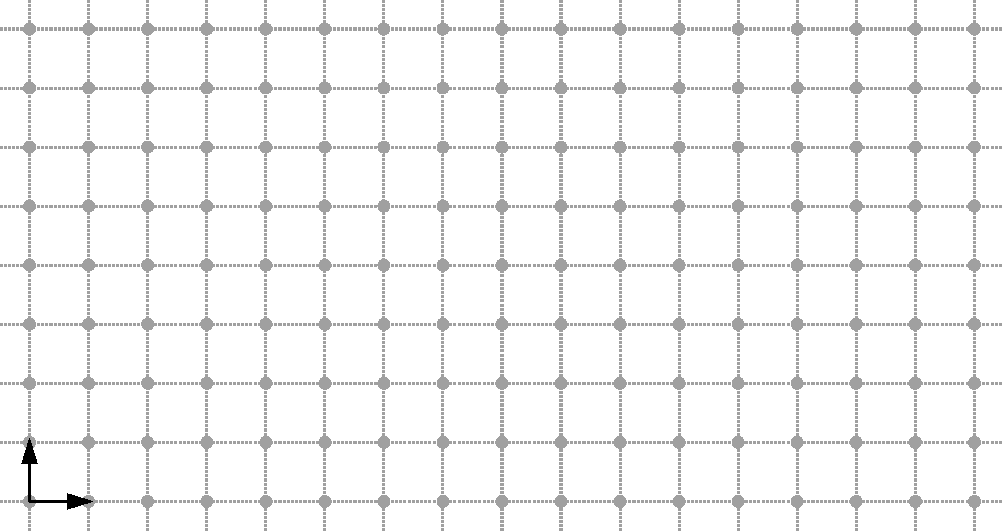
\includegraphics[width=10cm]{domain}\\ ~\\
    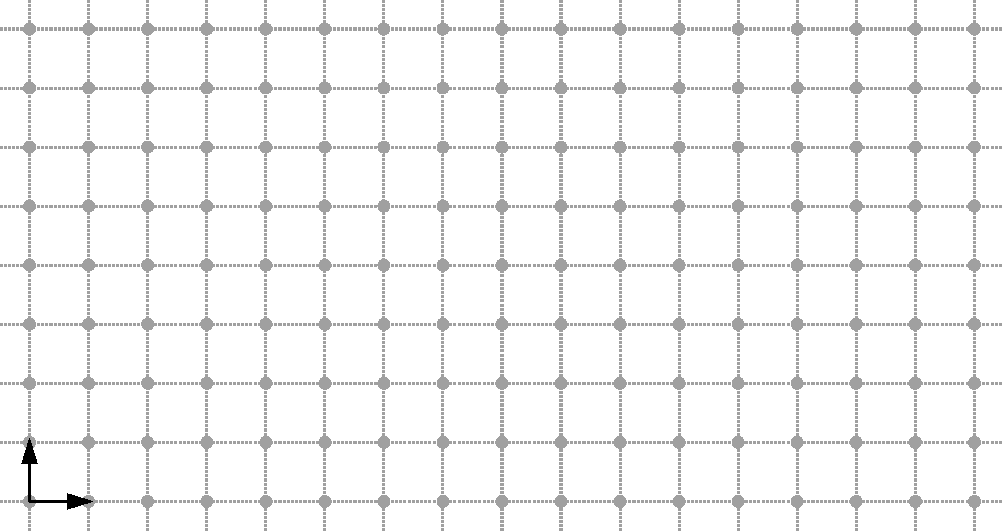
\includegraphics[width=10cm]{domain}
  \end{center}
\end{figure}




\end{document}

